\section{Domain understanding}
Questa è una delle fasi del processo $RE$, in particolare la prima da eseguire.\\
Approfondiamo questa fase analizzando i vari aspetti. Partiamo con la tecnica dell'\textbf{elicitation}, che consiste in tecniche atte allo scoprire requisiti che un progetto deve soddisfare. Bisonga iniziare dagli stakeholder.
\subsubsection{Stakeholders}
La prima parte è la selezione degli stakeholders del progetto.  In generale uno stakeholder è un'organizzazione o una persona che nutre un interesse rispetto al progetto. Conoscendo gli stakeholders avremo modo di prendere in considerazioni gli interessi degli stakeholders tramite diverse strategie. Idealmente si vuole realizzare qualcosa che soddisfi tutti gli interessi di tutti gli stakeholders esistenti. Difficile dire se sono stati presi in considerazione tutti gli stakeholders per il nostro applicativo.
Ci sono diversi aspetti da considerare per la selezione degli stakeholders:
\begin{itemize}
  \item posizione nell'organizzazione
  \item ruolo nel prendere decisioni sul \textit{system-to-be}
  \item livello di esperienza del dominio applicativo
  \item esposizione al problema che il sistema deve risolvere
  \item influenza nell'accettazione del sistema
  \item obiettivi personali ed eventuali conflitti di interesse dei componenti coinvolti 
\end{itemize}
Si ha che gli stakeholders che non fanno dell'organizzazione ma che magari hanno a che fare con associazioni, addetti alle normative di settore e altro, producendo un insieme molto ampio e variegato, proporzionalmente alla grandezza del progetto. Si hanno anche stakeholders che non interagiscono direttamente col sistema.\\ 
Un modo per identificare gli stakeholders è tramite una serie di semplici domande, tramite una piccola attività di brainstorming (da fare anche insieme ad analisti), le domande possono essere le seguenti (questa è una sorta di check-list):
\begin{itemize}
  \item chi è influenzato positivamente e negativamente dal progetto? 
  \item chi ha il potere di fargli avere successo (o farlo fallire)? 
  \item chi prende le decisioni in materia di denaro? 
  \item chi sono i fornitori? 
  \item chi sono gli utenti finali? 
  \item chi ha influenza, anche indiretta, sugli altri stakeholder? 
  \item chi potrebbe risolvere potenziali problemi con il progetto? 
  \item chi si occupa di assegnare o procurare risorse o strutture? 
  \item chi ha competenze specialistiche cruciali per il progetto?
\end{itemize}
Dimenticare uno stakeholders può portare ritardi o fallimenti del progetto, dovendo rivedere magari requisti (specifici di quello stakeholder) o dovendo rifare parti di sviluppo. Questa fase è quindi da non sottovalutare per non rischiare di non implementare requisiti solo per il semplice fatto di non aver incluso tra gli stakeholders una figura caratterizzate. Si hanno varie difficoltà nell'acquisire informazioni dagli stakeholders, rendendo complesso il dialogo:
\begin{itemize}
  \item fonti di conoscenza sul sistema distribuite sui vari stakeholders e tali fonti spesso sono contrastanti 
  \item accesso difficile alle fonti 
  \item ostacoli alla buona comunicazione, avendo background diversi sul dominio
  \item conoscenza non comunicata esplicitamente (magari anche solo perché date per scontate dagli esperti di un certo dominio o perché alcune informazioni sono sensibili o segretate) e bisogni nascosti
  \item fattori socio-politici 
  \item condizioni instabili e mutabili, cambiano gli stakeholders, si hanno dinamiche aziendale mutevoli e cambi di ruoli.
\end{itemize}
Serve molta esperienza per gestire queste situazioni.\\
Servono quindi \textbf{buone capacità comunicative}, sapendo usare la giusta terminologia di dominio (ovvero quella dello stakeholders), arrivando dritti al punto e instaurare un rapporto di fiducia con gli stakeholders.\\ Si ha inoltre un piccola pratica, detta \textit{knowledge reformulation}, ovvero quando si acquisiscono informazioni anche da fonti multiple è bene riformulare tale informazione allo stakeholder, per verificare una corretta comprensione.\\
È bene fare distinzione sulle tecniche di engagement con gli stakeholders, data la loro numerosità, considerando due variabili rappresentanti il potere decisionale, queste possono assumere valore $low$ e $high$. Le due variabili sono: 
\begin{enumerate}
  \item potere decisionale
  \item interesse nel progetto
\end{enumerate}
Da quanto detto, possiamo riassumere la strategia attraverso una tabella:
\begin{table}[H]
\centering
    \begin{tabular}{|p{0.1\linewidth}|p{0.1\linewidth}|p{0.8\linewidth}|}
    \hline
    \textbf{Power} &
      \textbf{Interest} &
      \textbf{Strategy} \\ \hline
    High &
      High &
      \textbf{fully engage}: ovvero coinvolgimento regolare degli stakeholders che in questo caso sono della categoria principale. Devono essere estremamente soddisfatti \\ \hline
    High &
      Low &
      \textbf{keep satisfied}: se hanno alto potere decisionale si cerca di mantenerli informati e soddisfatti ma senza troppi dettagli \\ \hline
    Low &
      High &
      \textbf{keep satisfied}: se hanno alto interesse, essendo spesso gli end-user, si cerca di consultarli spesso cercando di risolvere le problematiche indicate, coinvolgendoli regolarmente per ottenere dettagli e informazioni specifiche, essendo spesso i più informati sui dettagli \\ \hline
    Low &
      Low &
      \textbf{minimum effort}: mentendoli informati in modo generale e  monitorandone eventuali cambi di ruolo, potere o interesse \\ \hline
    \end{tabular}
\end{table}
In seguito alla decisione degli stakeholders possiamo passare alle tecniche di elicitation.

\subsection{Elicitation techniques}
Si hanno due famiglie principali:
\begin{itemize}
  \item \textbf{artefact-driven}, che fanno uso di artefatti per poter scoprire requisiti
  \item \textbf{stakeholders-driven}, che fanno invece uso degli stakeholders
\end{itemize}
\subsubsection{Artefact-driven}
La prima fase, molto fondamentale, è il \textbf{background study}, ovvero collezionare leggere e sintetizzare la conoscenza che viene dai documenti su:
\begin{itemize}
  \item le \textbf{organizzazioni stesse}, ovvero grafici, business plan, report finanziari, tempi delle riunioni etc$\ldots$
  \item il \textbf{dominio applicativo}, ovvero libri, paper, report su sistemi simili etc$\ldots$
  \item il funzionamento del \textbf{system-as-is}, ovvero workflow documentati, procedure, regole di business, report di errori, richieste di cambiamenti etc$\ldots$
\end{itemize}
Queste collezioni di dati ci permettono di informarci in modo autonomo sul mondo in cui si andrà a lavorare, senza coinvolgere lo stakeholders, in quanto costoso, dispendioso e limitato in termini di tempo. Gli stakeholders vanno interpellati non per informazioni reperibili autonomamente ma per estrarre conoscenza non pubblica e non documentata. Ci si presenta allo stakeholder già con una base di conoscenza e conoscendo già la terminologia corretta del dominio. Inoltre loro non sono sempre presenti per rispondere alle nostre domande\\
Si ha quindi l'attività di \textbf{data collection} dove si estraggono informazioni, ma non più dai documenti, ma dai dati di marketing, costi e altro. Sono dati utili per studiare il target. Si possono fare attività di \textit{survey}. Si collezionano dati anche già documentati.\\

L'attività di background study ha ovviamente dei limiti di scalabilità, non potendo leggere troppe cose, sia per tempo che per costo. In questa fase è ottimo sfruttare la \textit{meta-knowledge}, usando anche le conoscenze che si hanno già,  per selezionare le parti dei documenti più rilevanti. L'aspetto principale di questa fase rimane quello di poter produrre informazioni utile per l'interazione con gli stakeholders.\\ 

Un'altra tecnica è quella dei \textbf{questionari}, ovvero una lista di quesiti, che hanno una lista di possibile risposte,  da presentare a stakeholders senza fare distinzione tra loro (ognuno ha esigenze diverse da non sottovalutare). Si possono così interrogare molti stakeholders contemporaneamente. Le domande devono essere ben espresse, in modo che non ci siano ambiguità e che non comportino problematiche nella risposta. Si hanno quindi domande spesso a risposta multipla (per capire se fare nel modo A o B, ad esempio) e raramente domande aperte, che spesso vengono ignorate o mal risposte, ed eventualmente con risposte pesate, per indicare il livello di gradimento.\\

È bene fare pochi questionari efficaci, con risposte poco affette da rumore. Si deve avere una numerosità di domande adeguata. Spesso si usa prima un piccolo campione ai quali somministrare il questionario per poi inviarlo a tutti. Questi questionari aiutano a preparare colloqui/interviste mirati più efficaci (il questionario non è un'alternativa all'intervista).\\  

Il questionario deve essere preparato con cura, questo perché si devono evitare ambiguità e inserimenti di bias (esempio: central bias) nelle domande. Le domande non devono condizionare la risposta. La raggiungibilità dei soggetti scelti è essenziale, nonché la scelta degli stessi. È buona pratica avere domande di \textit{cross-check} (magari due domande che chiedono la cosa opposta) per controllare chi sta rispondendo non dia risposte inconsistenti e incoerenti, sintomo del fatto che uno non risponda a caso.\\

Un altro tipo di artefatto usato sono le \textbf{storyboards}, ovvero narrazioni, tramite esempi, di uso del sistema, sia del \textit{system-as-is} che del \textit{system-to-be} . Sono quindi storie fatte tramite sequenze di snapshots (slide, figure, sketch etc$\ldots$) che ci mostrano cosa viene mostrato e a che cosa serve. Tali storie si creano in due modi:
\begin{enumerate}
  \item \textbf{modo passivo}, dove si narra la storia costruita allo stakeholder
  \item \textbf{modo attivo}, dove lo stakeholder contribuisce alla costruzione della narrazione
 \end{enumerate}
Ovviamente vengono fatte solo per i workflow chiare.\\
Legati alle storyboards si hanno gli \textbf{scenari} che descrivono, attraverso una sequenza di interazioni rappresentate con testi o diagrammi, l'utilizzo del sistema, sia \textit{as-is} che \textit{to-be}. L'uso di esempi rende semplice la comunicazione e l'interazione con gli altri. Si hanno diversi tipi di scenario:
\begin{enumerate}
    \item \textbf{positivo}, ovvero come il sistema si dovrebbe comportare, e si posso dividere in due categori di scenari:
    \begin{itemize}
        \item \textbf{normale}, ovvero tutto procede come dovrebbe
        \item \textbf{anormale}, ovvero cosa succede in casi eccezionali
    \end{itemize}
    \item \textbf{negativo}, ovvero cosa il sistema non dovrebbe fare
\end{enumerate}
[\textbf{NELLE SLIDE 18/19 VIENE MOSTRATO UN ESEMPIO}]\\
Gli scenari sono un metodo naturale di interazione con lo stakeholders e possono essere usati per guidare alla stesura di \textbf{testi di accettazione}. Hanno comunque dei limiti, essendo solo esempi parziali, non descrivono come il sistema si deve comportare, e sono poco adatti alla combinazione tra essi. Gli esempi possono anche deviare la comprensione del sistema, che magari può comportarsi in molti altri modi, avendo anche dettagli irrilevanti. Gli scenari non si prestano all'interazione con molti stakeholder, a causa della variabilità di questi.\\

Un'altra tecnica è la costruzione di \textbf{prototipi} e \textbf{mock-up}. In questo caso l'obiettivo è quello di controllare l'adeguatezza di un requisito, che viene mostrato in modo visuale nella sua ipotetica formula finale. Si hanno quindi piccoli esempi del software in azione, chiarendo e verificando che sia quello di cui l'utente ha bisogno. Ovviamente un mock-up non ha la logica applicative ma risposte costruite a priori. A seconda del tipo di mock-up, o per chi viene costruito, il focus viene indirizzato su: 
\begin{itemize}
  \item \textbf{funzionalità}, se sono state comprese correttamente e in modo esaustivo
  \item \textbf{UI e UX}, avendo focus più orientati all'usabilità 
\end{itemize}
Si parla di \textbf{mock-up} se dopo l'uso viene buttato e di \textbf{prototipo} se, in caso di approvazione, viene usato come base del software o comunque riutilizzato in qualche modo, fornendo eventualmente una base evolutiva del software finale.\\
\begin{figure}[H]
    \centering
    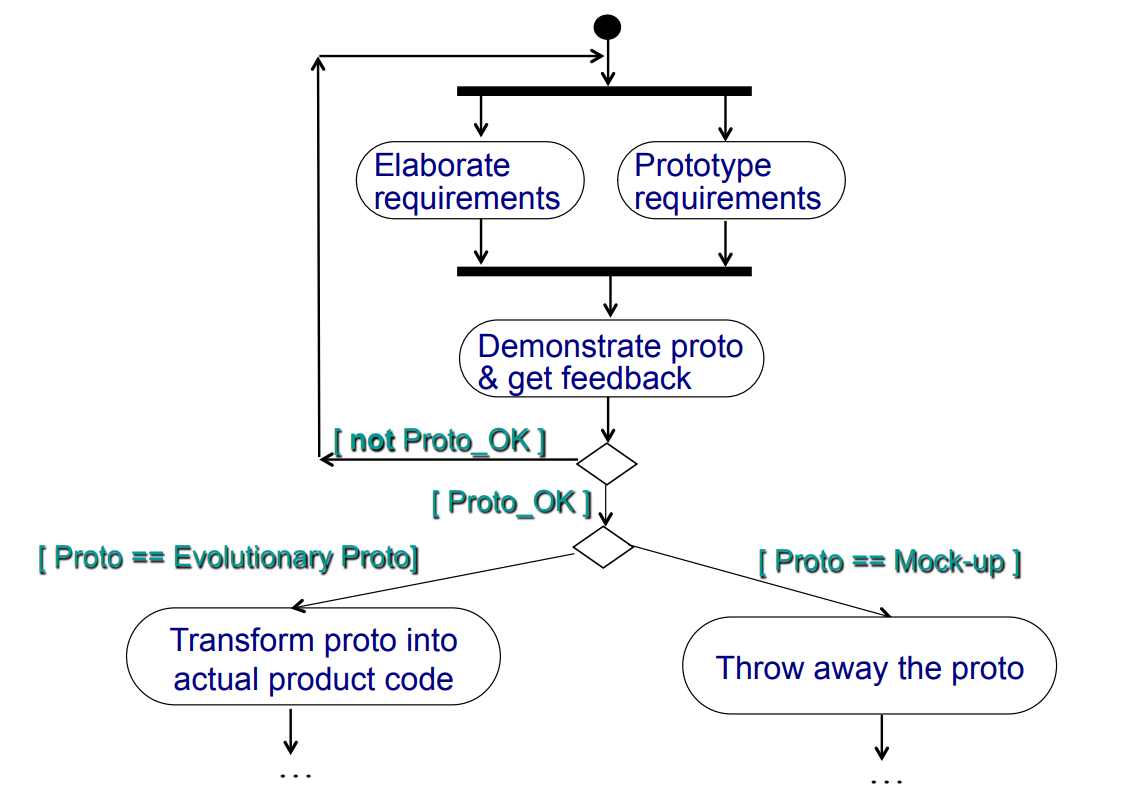
\includegraphics[scale = 0.5]{Imm/flowchartr.PNG}
    \caption{Prototipazione dei requisiti}
\end{figure}
Come pro si ha una sensazione di concretezza per lo stakeholder, anche visuale, permettendo anche già una sorta di training sul software che si produce. Purtroppo spesso i m mock-up sono costosi, inoltre la loro natura simulata può produrre aspettative troppo alte, magari anche solo in termini di prestazioni (il mock-up è super performante mentre il prodotto finale molto meno, avendo tutta la logica applicativa sotto, ad esempio attesa di risposta da un database). Inoltre in un'ottica di riuso un mock-up è spesso inutilizzabile a causa del \textbf{quick-and-dirty code}.

Si ha anche il \textbf{knowledge reuse}, per velocizzare l'elicitation, riusando conoscenze pregresse da sistemi simili a quello sotto studio.\\
Si hanno 3 fasi:
\begin{enumerate}
  \item \textbf{retrieve}: trarre conoscenze e informazioni rilevanti da altri sistemi
  \item \textbf{transpose}: riportare le conoscenze acquisite nel sistema in studio
  \item \textbf{validate, adapt, integrate}, ovvero convalidare il risultato, adattarlo se necessario e integrarlo con la
  conoscenza del sistema già acquisita
\end{enumerate}
Le conoscenze possono essere dipendenti o indipendenti dal dominio.\\
Per quelle indipendenti dal dominio viene utilizzata una tassonomia presente nella slide 26. La tassonomia abbiamo visto che veniva rappresentata attraverso un albero, per ogni nodo o foglia ci poniamo nell'ottica di chiederci se, dal requisito rappresentato nel nodo, possiamo ricavare requisiti di istanza. \\
Sia ad esempio preso in cosiderazione il tempo di risposta, possiamo chiederci: tempo di risposta per cosa? partecipanti? notifica di un meeting?\\
Per quelle dipendenti dal dominio quello che facciamo è eseguire la specializzazione trasformando gli oggetti astratti in oggetti concreti all'interno del sistema. 

Si hanno i seguenti pro:
\begin{itemize}
  \item analisti esperti riutilizzano naturalmente dall'esperienza passata
  \item riduzione degli sforzi di eliciation
  \item ereditarietà della struttura e qualità delle specifiche del dominio astratto 
  \item efficace per completare i requisiti con aspetti trascurati
\end{itemize}
e i seguenti contro:
\begin{itemize}
  \item efficace solo se il dominio astratto è sufficientemente simile e  accurato 
  \item definire domini astratti per una riusabilità significativa è difficile 
  \item si hanno forti sforzi di convalida e integrazione 
  \item le corrispondenze vicine possono richiedere adattamenti complicati
\end{itemize}

Ci sono altri metodi artefact-driven:
\begin{itemize}
    \item \textbf{Card Sort}, si chiede agli stakeholders di posizionare i cartoncini che rappresentano concetti, in modo testuale o grafico. Si chiede poi di classificarli per somiglianza all'interno di un subset, usando i loro criteri di valutazione.(es: sotto un subset "Fitness" associamo i cartoncini "Workout", "Hydration") \\ Per ogni subset viene chiesto le proprietà utilizzate per il raggruppamento. Questo viene eseguito in modo iterativo per nuovi gruppi/nuove proprietà. Come obiettivo vogliamo acquisire nuove informazioni sul concetto già appreso. 
    \item \textbf{Data collection} avevamo detto che si usano dati di marketing, e come obiettivo quello di raccogliere fatti e figure. Questo viene fatto attraverso l'uso dei dati che sono esposti pubblicamente dall'azienda. 
\end{itemize}

\subsubsection{Stakeholders-driven}
Passiamo quindi alle tecniche in cui interagisce direttamente lo stakeholder, senza la mediazione di artefatti.\\
La principale tecnica è l'\textbf{intervista} che consiste in:
\begin{itemize}
  \item selezione mirata dello stakeholder, in base alle informazioni necessarie
  \item fare l'intervista registrando le risposte
  \item scrivere il \textit{transcript} dell'intervista e produrre subito il report
  \item sottomettere all'intervistato il report per validazione
\end{itemize}
Si può avere un'intervista anche con più stakeholder (perdendo però in parte la costruzione del rapporto personale con lo stakeholder). L'intervista è una tecnica costosa e le interviste possono essere poche, bisogna quindi procedere in modo attento.\\

Si hanno due tipi diversi di interviste:
\begin{enumerate}
  \item \textbf{interviste strutturate}, dove si parte con un insieme di domande già scelto per un certo obiettivo. Si da poco spazio ad una discussione aperta
  \item \textbf{interviste non strutturate}, dove si da spazio alla discussione aperta e libera sul \textit{system-as-is}, sulle problematiche e sulle possibili soluzioni. 
\end{enumerate}
Spesso si hanno interviste miste, nella prima parte strutturate e poi con domande e argomenti liberi. Gli argomenti vanno calibrati così come il numero di domande, per evitare perdite di tempo e di perdità di concentrazione da parte dello stakeholder.\\
Vediamo quindi qualche linea guida per la preparazione delle interviste.
\begin{itemize}
  \item bisogna arrivare preparati, tramite il background study, evitare domande ovvie per l'intervista.
  \item per costruire un rapporto con lo stakeholder le domande devono essere su  misura dello stesso, in base al suo lavoro e ruolo
  \item mettere in centro all'intervista necessità e problematiche dell'intervistato, chiarendo di essere interessati al suo punto di vista
  \item evitare che la discussioni dilaghi su argomenti inutili
  \item fare in modo che l'intervistato si senta a suo agio, magari iniziando con qualche chiacchiera informale e domande semplici per poi spostarsi su domande difficili
  \item dimostrarsi affidabile
  \item chiedere sempre perché qualcosa vada fatto, questo per conoscere la motivazione che ha lo stakeholder riguardo la creazione del applicativo
  \item evitare domande bias che influenzino la risposta
  \item evitare domande a cui sicuramente l'intervistato non sa rispondere
\end{itemize}

Nel transcript bisogna includere reazioni personali (anche se queste parti possono essere tolte dalla copia di validazione).\\
Si hanno modi alternativi per interagire con lo stakeholder. Talvolta si ha bisogno anche di altre modalità oltre la sola intervista.\\
Spesso è più facile infatti far osservare che descrivere a parole e quindi si hanno \textbf{studi osservazionali e etnografici}, ovvero studi che si basano sull'osservazione degli stakeholders all'azione osservando come svolgono vari task per cogliere problemi e funzionalità. Si hanno due modalità di osservazione:
\begin{enumerate}
  \item \textbf{osservazione passiva}, dove non si produce interferenza sulle azioni dello stakeholder, guardando da fuori, registrando record e producendo un transcript. Si hanno due particolari \textbf{osservazioni passive}:
      \begin{enumerate}
        \item \textbf{protocol analysis}, dove si osserva qualcuno che svolge un certo task (la slide dice che viene contemporaneamente spiegato)
        \item \textbf{ethnographic studies}, studio che si svolge in un lungo periodo di tempo, dove si prova a scoprire le proprietà emergenti del gruppo sociale coinvolto
      \end{enumerate}
  \item \textbf{osservazione attiva}, dove si svolge in prima persona i task, diventando eventualmente team member, capendo attivamente come deve essere svolto un task
\end{enumerate}
Gli studi osservazionali aiutano a scoprire requisti che restano altrimenti taciti e a scoprire problemi nascosti, che non si noterebbero nell'intervista. Aiuta anche a contestualizzare le informazioni. È comunque un'operazione lenta e costosa, dovendo recarsi di persona ad osservare ed annotare. Può essere potenzialmente inaccurato in quanto una persona conscia di essere osservata potrebbe comportarsi in modo diverso. L'osservazione si focalizza comunque solo sul \textit{system-as-is} e non aiuta molto nel \textit{system-to-be}.\\

Si hanno altri modi di interazione con gli stakeholders tra cui le \textbf{group sessions}, ovvero una famiglia di tecniche utili per la risoluzione di conflitti. L'elicitation prende la forma di un workshop di uno o più giorni in cui si ha una discussione tra vari partecipanti scelti in modo dipendente a seconda dall'obiettivo, innescando una discussione utile a comprendere il \textit{system-to-be}. Mettendo insieme le parti con visioni conflittuali si possono risolvere diversi problemi. Su hanno due tipologie di \textit{group sessions}:
\begin{enumerate}
  \item \textbf{strutturate} dove ogni partecipante ha un ruolo chiaramente definito: leader, moderatore, manager, utente, sviluppatore o altro. Ognuno contribuisce in funzione del ruolo, permettendo di ragionare su requisiti di più alto livello, comuni a più figure, e su conflitti ad alto livello
  \item \textbf{non strutturate}, dette anche \textbf{sessioni brainstorming}, dove i partecipanti non hanno un ruolo definito. La sessione è formata da due fasi:
  \begin{enumerate}
    \item \textbf{generazione delle idee}, dove tutti espongono le proprie idee in merito al problema/conflitto che ha generato la sessione
    \item \textbf{valutazione delle idee}, dove tutte le idee vengono analizzate una per una e valutate per valore, costo, fattibilità e altri parametri da prendere in considerazione in modo da arrivare una visione condivisa sugli approcci da usare secondo una certa prioritizzazione
  \end{enumerate}
\end{enumerate}
Si ha il pro di poter esplorare varie opzioni e a portare a risoluzioni sfruttando anche l'inventiva dei partecipanti. La composizione del gruppo è comunque critica, molti potrebbero non avere tempo, alcuni potrebbero prendere posizioni dominanti introducendo bias, condizionando la discussione e le decisioni. Si rischia inoltre che la discussione diverga verso inutilità senza convergere sugli aspetti per cui è stata convocata la sessione.\\ \textbf{Ogni attività, sia artefact-driven che stakeholder-driven viene svolta solo se si hanno chiari gli obiettivi che si vogliono ottenere con tale attività.}
